% Appendix B

\chapter{Computing Flight Profiles}
\label{AppendixB}

For the given equipment type, let $r_A$ denote the rate of ascent and $r_D$ the rate of descent, both in feet per second. Let $a_C$ denote the cruising altitude in feet. Let $t_A=a_C/r_A$, the time taken to ascend to cruising altitude and $t_D=a_C/r_D$, the time taken to descend from cruising altitude, both in seconds. Let $t_C$ denote the time spent at cruising altitude, after ascent and before descent and let $t_T=t_A+t_C+t_D$ denote the total flight time. It is possible on short trips that the aircraft does not reach cruising altitude before needing to begin its descent. We assume it continues to ascend until it reaches its peak altitude at which time it must begin its descent. Denote this altitude by $a_M$, in feet. Let $t_M=a_M/r_A$ denote the time taken to ascend to peak altitude and $t_R=a_M/r_D$ the residual time to descend from this altitude to complete the trip. In this case, $t_T=t_M+t_R$. Figure \ref{fig:SpeedModel} illustrates for the typical case in which $a_M$ exceeds $a_C$.

\begin{figure}[htbp]
    \centering
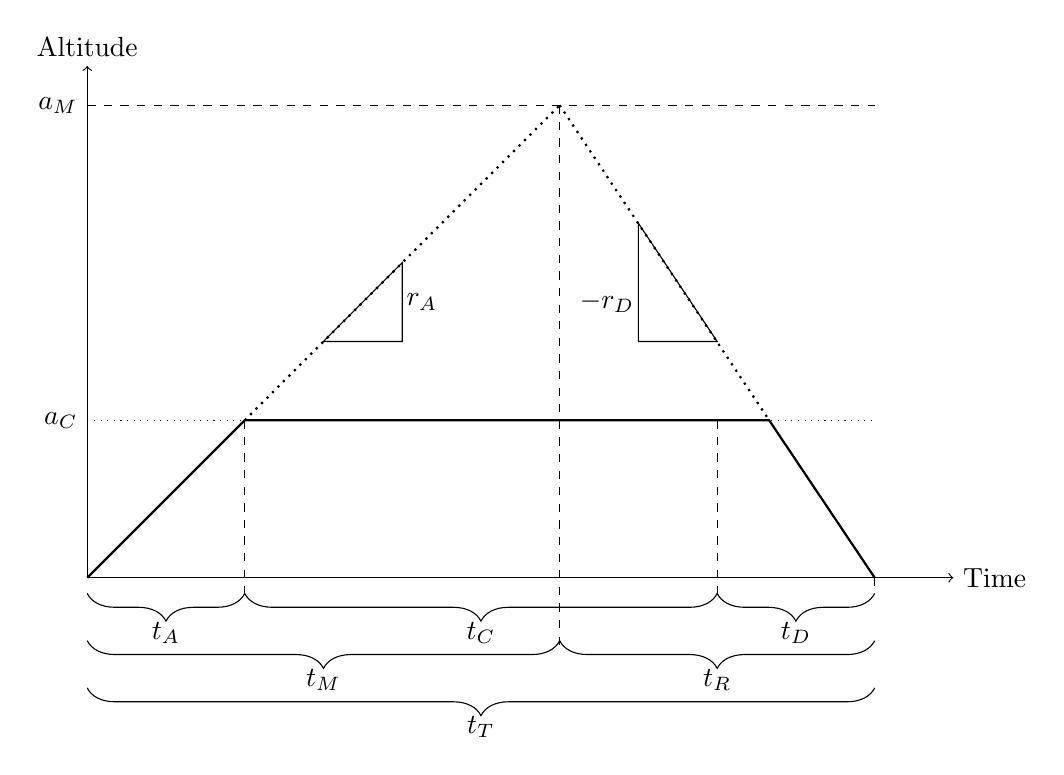
\begin{tikzpicture}

% Axes
\draw[->] (0,0) -- (11,0) node[right] {Time};
\draw[->] (0,0) -- (0,6.5) node[above] {Altitude};

% Dotted lines and labels for altitude levels
\draw[dashed] (0,6) -- (10,6);

%\tikz[baseline=(todotted.base)]\path[red, dash dot dot,transform canvas={yshift=-2pt}] node  (todotted) {} edge ([xshift=2cm]todotted){};
\draw[dotted] (0,2) -- (10,2);
\node[left] at (0,6) {$a_M$};
\node[left] at (0,2) {$a_C$};
\draw[dotted,thick] (2,2) -- (6,6);
\draw[dotted,thick] (6,6) -- (8.66,2);
% Solid lines and triangle sides
\draw[thick] (0,0) -- (2,2) -- (8.66,2) -- (10,0);
\draw[dashed] (2,2) -- (2,-0.3);
\draw[dashed] (8,2) -- (8,-0.3);
\draw[dashed] (6,6) -- (6,-0.9);
\draw[dashed] (10,0) -- (10,-0.2);
% Right angle symbols
\draw (3,3) -- (4,3) -- (4,4)  -- cycle;
\draw (8,3) -- (7,3) -- (7,4.5)  -- cycle;

% Altitude segments
\node at (4.25,3.5) {$r_A$};
\node at (6.6,3.5) {$-r_D$};

% Braces and labels for time segments
\draw[decorate,decoration={brace,amplitude=10pt,mirror}] (0,-0.2) -- (2,-0.2) node[midway,yshift=-0.5cm] {$t_A$};
\draw[decorate,decoration={brace,amplitude=10pt,mirror}] (2,-0.2) -- (8,-0.2) node[midway,yshift=-0.5cm] {$t_C$};
\draw[decorate,decoration={brace,amplitude=10pt,mirror}] (8,-0.2) -- (10,-0.2) node[midway,yshift=-0.5cm] {$t_D$};

\draw[decorate,decoration={brace,amplitude=10pt,mirror}] (0,-1.4) -- (10,-1.4) node[midway,yshift=-0.5cm] {$t_T$};
\draw[decorate,decoration={brace,amplitude=10pt,mirror}] (0,-0.8) -- (6,-0.8) node[midway,yshift=-0.5cm] {$t_M$};
\draw[decorate,decoration={brace,amplitude=10pt,mirror}] (6,-0.8) -- (10,-0.8) node[midway,yshift=-0.5cm] {$t_R$};

\end{tikzpicture}
    \caption{Graph of Idealized Altitude \textit{vs.} Time Profile of Typical Flight}
    \label{fig:SpeedModel}
\end{figure}

Let $s(t)$ denote the speed of the aircraft over the course of its journey, in nautical miles per second and $s_C$ the cruising speed in nautical miles per second (all time is measured in seconds). We assume that the rate of acceleration is constant during ascent and the rate of deceleration is constant during descent. In the typical case (that is, when $a_M\geq a_C$), that leads to the formula:

\begin{equation*}
s(t)=\left\{
    \begin{array}{ll}
      \frac{t}{t_A}s_C, & \mbox{if $0\leq t \leq t_A$.}\\
      s_C, & \mbox{if $t_A< t \leq t_A+t_C$,}\\
	\frac{t_T-t}{t_D}s_C, & \mbox{if $t_A+t_C< t \leq t_T$.}
    \end{array}
  \right.
\end{equation*}

In the atypical case ($a_M < a_C$), the aircraft does not reach its cruising speed at its peak altitude. Assuming constant acceleration, it reaches a speed of $s(t_M)=\frac{a_M}{a_C}s_C$. Consequently, the formula for $s(t)$ in the atypical case is given by:

\begin{equation*}
s(t)=\left\{
    \begin{array}{ll}
      \frac{ta_M}{t_Ma_C}s_C, & \mbox{if $0\leq t \leq t_M$.}\\
	\frac{(t_T-t)a_M}{t_Ra_C}s_C, & \mbox{if $t_M< t \leq t_T$,}
    \end{array}
  \right.
\end{equation*}

Let $d(t)=\int\limits_0^t s(u)du$, the distance covered in the time interval $[0,t]$, in nautical miles. Let $d_A=d(t_A)$ denote the distance covered during the ascent portion of flight, $d_C=d(t_A+t_C)-d_A$, the distance covered during cruise, and $d_D=d(t_T)-d_A-d_C$, the distance covered during descent, in the typical case. In the atypical case, let $d_M=d(t_M)$ denote the distance covered until peak altitude $a_M$ is reached and let $d_R=d(t_T)-d_M$ denote the distance covered during descent from $a_M$. Let $d_T=d(t_T)$ denote the total distance covered under either case ($d_T=d_A+d_C+d_D$ in the typical case and $d_T=d_M+d_R$ in the atypical case). The following results are easily verified:

\begin{lemma}
Under the assumption of constant acceleration and deceleration, the critical distances in the trajectory plan are given by:
\begin{align*}
d_A&=\frac{a_C}{2r_A}s_C,\\
d_C&=t_Cs_C, \\
d_D&=\frac{a_C}{2r_D}s_C,\\
d_M&=\frac{a_M^2}{2a_Cr_A}s_C, \mbox{ and}\\
d_R&=\frac{a_M^2}{2a_Cr_D}s_C.
\end{align*}
\end{lemma}
\begin{proof}
In the typical case, for $t\leq t_A$, we have:

\begin{equation*}
d(t)=\int\limits_0^t \frac{u}{t_A}s_C du=\frac{t^2}{2t_A}s_C.
\end{equation*}

Hence, 

\begin{equation*}
d_A=d(t_A)=\frac{t_A^2}{2t_A}s_C=\frac{t_A}{2}s_C=\frac{a_C}{2r_A}s_C.
\end{equation*}

Similarly,
\begin{equation*}
d_D=\int\limits_{t_T-t_D}^{t_T} \frac{t_T-u}{t_D}s_C du=\int\limits_0^{t_D} \frac{x}{t_D}s_C dx=\frac{t_D^2}{2t_D}s_C=\frac{t_D}{2}s_C=\frac{a_C}{2r_D}s_C.
\end{equation*}

In the atypical case, for $t\leq t_M$:
\begin{equation*}
d(t)=\int\limits_0^t \frac{ua_M}{t_Ma_C}s_C du=\frac{t^2a_M}{2t_Ma_C}s_C
\end{equation*}

Hence, 

\begin{equation*}
d_M=d(t_M)=\frac{t_M^2a_M}{2t_Ma_C}s_C=\frac{t_Ma_M}{2a_C}s_C=\frac{a_M^2}{2a_Cr_A}s_C.
\end{equation*}

Similarly,
\begin{equation*}
d_R=\int\limits_{t_T-t_R}^{t_T} \frac{(t_T-u)a_M}{t_Ra_C}s_C du=\int\limits_0^{t_R} \frac{xa_M}{t_Ra_C}s_C dx=\frac{t_R^2a_M}{2t_Ra_C}s_C=\frac{t_Ra_M}{2a_C}s_C=\frac{a_M^2}{2a_Cr_D}s_C.
\end{equation*}
$ \blacksquare $

\end{proof}

Let $\bar{D}$ denote the distance between an arbitrary origin-destination pair of airports. In the typical case, that would imply that $d_C=\bar{D}-d_A-d_D$. Hence,

\begin{align*}
d_C&=\bar{D}-\frac{a_Cs_C}{2}(\frac{1}{r_A}+\frac{1}{r_D})\\
&=\bar{D}-\frac{a_Cs_C}{2}\Big(\frac{r_D+r_A}{r_Ar_D}\Big)
\end{align*}

Provided $d_C\geq 0$, this leads to the following:

\begin{align*}
t_T&= t_A+t_D+t_C\\
&=\frac{a_C}{r_A}+\frac{a_C}{r_D}+\frac{d_C}{s_C}\\
&=a_C\big(\frac{r_D+r_A}{r_Ar_D}\big)+\frac{\bar{D}}{s_C}-\frac{a_C}{2}\Big(\frac{r_D+r_A}{r_Ar_D}\Big)\\
&=\frac{\bar{D}}{s_C}+\frac{a_C}{2}\Big(\frac{r_D+r_A}{r_Ar_D}\Big)
\end{align*}

In the atypical case, $a_M$ would need to satisfy the equation $d_M+d_R=\bar{D}$. Hence,

\begin{align*}
\frac{a_M^2}{2a_Cr_A}s_C+\frac{a_M^2}{2a_Cr_D}s_C &=\bar{D}\\
\frac{s_C}{2a_C}(\frac{1}{r_A}+\frac{1}{r_D})a_M^2 &=\bar{D}\\
a_M^2&=\frac{2\bar{D}a_C}{s_C}\Big(\frac{r_Ar_D}{r_D+r_A}\Big)
\end{align*}

For a given origin-pair distance, $\bar{D}$, the critical points of the atypical flight trajectory are thus given by:

\begin{align*}
d_M &= \frac{\bar{D}}{r_A}\Big(\frac{r_Ar_D}{r_D+r_A}\Big)\\
d_R&= \frac{\bar{D}}{r_D}\Big(\frac{r_Ar_D}{r_D+r_A}\Big)
\end{align*}

and the total time is given by:

\begin{align*}
t_T&=t_M+t_R\\
&=\frac{a_M}{r_A}+\frac{a_M}{r_D}\\
&=a_M\Big(\frac{r_D+r_A}{r_Ar_D}\Big)\\
&=\sqrt{\frac{2\bar{D}a_C}{s_C}\Big(\frac{r_D+r_A}{r_Ar_D}\Big)}
\end{align*}

The condition of atypicality, $a_M\leq a_C$, is equivalent to the condition $d_C\leq 0$. 

\begin{proposition}
Under the assumption of constant acceleration and deceleration, the distance-time profile $d(t)$ when the given origin-destination pair distance, $\bar{D}$ satisfies $\bar{D}\geq \frac{a_Cs_C}{2}\Big(\frac{r_D+r_A}{r_Ar_D}\Big)$ is given by:

\begin{equation*}
d(t)=\left\{
    \begin{array}{ll}
   \frac{t^2r_A}{2a_C}s_C, & \mbox{if $0\leq t \leq t_A$.}\\
d_A+(t-t_A)s_C,& \mbox{if $t_A\leq t \leq t_A+t_C$.}\\
	\bar{D}- \frac{(t_T-t)^2r_D}{2a_C}s_C, & \mbox{if $t_A+t_C< t \leq t_T$.}
    \end{array}
  \right.
\end{equation*}

When the condition is not satisfied, the distance-time profile is given by:

\begin{equation*}
d(t)=\left\{
    \begin{array}{ll}
   \frac{t^2r_A}{2a_C}s_C, & \mbox{if $0\leq t \leq t_M$.}\\
	\bar{D}- \frac{(t_T-t)^2r_D}{2a_C}s_C, & \mbox{if $t_M< t \leq t_T$.}
    \end{array}
  \right.
\end{equation*}

\end{proposition}
\begin{proof}
As an example of the calculations, when $t>t_M$, we have:
\begin{align*}
d(t)&=d_M+\int\limits_{t_M}^t \frac{(t_T-u)a_M}{t_Ra_C}s_C du\\
&= d_M+\int\limits_{t_T-t}^{t_T-t_M} \frac{xa_M}{t_Ra_C}s_C dx\\
&=d_M+\frac{x^2a_M}{2t_Ra_C}s_C\Big|_{t_T-t}^{t_T-t_M}\\
&=d_M +\frac{(t_T-t_M)^2a_M}{2t_Ra_C}s_C-\frac{(t_T-t)^2a_M}{2t_Ra_C}s_C\\
&=d_M +\frac{t_Ra_M}{2a_C}s_C-\frac{(t_T-t)^2a_M}{2t_Ra_C}s_C\\
&=d_M +\frac{a_M^2}{2r_Da_C}s_C-\frac{(t_T-t)^2r_D}{2a_C}s_C\\
&=d_M + \frac{\bar{D}}{r_D}\Big(\frac{r_Ar_D}{r_D+r_A}\Big)-\frac{(t_T-t)^2r_D}{2a_C}s_C\\
&=d_M+d_R-\frac{(t_T-t)^2r_D}{2a_C}s_C\\
&=\bar{D}- \frac{(t_T-t)^2r_D}{2a_C}s_C.
\end{align*}
\end{proof}
$\blacksquare$

Let $t(d)=d^{-1}(d)$, the time in seconds required to traverse $d$ nautical miles using the trajectory for the given origin-destination pair distance, $\bar{D}$.

\begin{corollary}
Under the assumption of constant acceleration and deceleration, the time-distance profile $t(d)$ when the given origin-destination pair distance, $\bar{D}$ satisfies $\bar{D}\geq \frac{a_Cs_C}{2}\Big(\frac{r_D+r_A}{r_Ar_D}\Big)$ is given by:

\begin{equation*}
t(d)=\left\{
    \begin{array}{ll}
     \sqrt{\frac{2a_Cd}{r_As_C}}, & \mbox{if $0\leq d \leq d_A$.}\\
\frac{a_C}{r_A}+\frac{(d-d_A)}{s_C},& \mbox{if $d_A\leq d \leq d_A+d_C$.}\\
	\frac{a_C}{r_A}+\frac{d_C}{s_C}+\frac{a_C}{r_D}-\sqrt{\frac{2a_C(\bar{D}-d)}{r_Ds_C}}, & \mbox{if $d_A+d_C< d \leq \bar{D}$.}
    \end{array}
  \right.
\end{equation*}
When the condition is not satisfied, the time-distance profile is given by:
\begin{equation*}
t(d)=\left\{
    \begin{array}{ll}
     \sqrt{\frac{2a_Cd}{r_As_C}}, & \mbox{if $0\leq d \leq d_M$.}\\
	\sqrt{\frac{2\bar{D}a_C}{s_C}\Big(\frac{r_D+r_A}{r_Ar_D}\Big)}-\sqrt{\frac{2a_C(\bar{D}-d)}{r_Ds_C}}, & \mbox{if $d_M< d \leq \bar{D}$.}
    \end{array}
  \right.
\end{equation*}
\end{corollary}



\begin{proof}
For example, when $d_A+d_C\leq d \leq \bar{D}$, or when $d_M<d\leq \bar{D}$:

\begin{align*}
	d&=\bar{D}- \frac{(t_T-t)^2r_D}{2a_C}s_C\\
\frac{(t_T-t)^2r_D}{2a_C}s_C&=\bar{D}-d\\
t&=t_T-\sqrt{\frac{2a_C(\bar{D}-d)}{r_Ds_C}}.
\end{align*}

Substituting for the two possible values of $t_T$ yields the result.

\end{proof}
$\blacksquare$

Figure \ref{fig:TimeVsDistance} illustrates the time-distance profile in the typical case ($a_M>a_C$) and Figure \ref{fig:TimeVsDistanceNoCruise} illustrates the time-distance profile in the atypical case when the aircraft does not reach cruising altitude before beginning its descent. Figure \ref{fig:SpeedScale} demonstrates how we compute minimum, maximum and preferred leg times ($t_{min}$, $t_{max}$ and $t_{pref}$, respectively) for a flight leg connecting waypoints at nautical mile 120 and nautical mile 180. The aircraft starts at 0m, gradually climbs to cruise height and attains the cruising altitude at 120nm, cruises from 120nm to 180nm, and continuously descends from 180nm to 200nm until landing. We assume a maximum speed-up of 5\% (scale=1.05) and a maximum slow-down of 10\% (scale=0.90).

\begin{figure}[htbp]
    \centering
    \includegraphics[width = 1\textwidth]{Figures/TimeVsDistance.png}
    \caption{Graph of Idealized Time vs. Distance Profile of Typical Flight}
    \label{fig:TimeVsDistance}
\end{figure}

\begin{figure}[htbp]
    \centering
    \includegraphics[width = 1\textwidth]{Figures/TimeVsDistanceNoCruise.png}
    \caption{Graph of Idealized Time vs. Distance Profile for Flight with No Cruise Portion}
    \label{fig:TimeVsDistanceNoCruise}
\end{figure}

\begin{filecontents}{data.dat}
 Distance	Time	 Scale1.00	Scale1.05	Scale0.90
2	146.9693846	146.9694	143.4274	154.9193
4	207.8460969	207.8461	202.837	219.089
6	254.5584412	254.5584	248.4236	268.3282
8	293.9387691	293.9388	286.8549	309.8387
10	328.6335345	328.6335	320.7135	346.4102
12	360	360	351.324	379.4733
14	388.8444419	388.8444	379.4733	409.878
16	415.6921938	415.6922	405.674	438.178
18	440.9081537	440.9082	430.2823	464.758
20	464.7580015	464.758	453.5574	489.8979
22	487.4423043	487.4423	475.695	513.8093
24	509.1168825	509.1169	496.8472	536.6563
26	529.905652	529.9057	517.135	558.5696
28	549.9090834	549.9091	536.6563	579.6551
30	569.2099788	569.21	555.4921	600
32	587.8775383	587.8775	573.7097	620
34	606	606	591.3665	640
36	624	624	608.5714	660
38	642	642	625.7143	680
40	660	660	642.8571	700
42	678	678	660	720
44	696	696	677.1429	740
46	714	714	694.2857	760
48	732	732	711.4286	780
50	750	750	728.5714	800
52	768	768	745.7143	820
54	786	786	762.8571	840
56	804	804	780	860
58	822	822	797.1429	880
60	840	840	814.2857	900
62	858	858	831.4286	920
64	876	876	848.5714	940
66	894	894	865.7143	960
68	912	912	882.8571	980
70	930	930	900	1000
72	948	948	917.1429	1020
74	966	966	934.2857	1040
76	984	984	951.4286	1060
78	1002	1002	968.5714	1080
80	1020	1020	985.7143	1100
82	1038	1038	1002.8571	1120
84	1056	1056	1020	1140
86	1074	1074	1037.1429	1160
88	1092	1092	1054.2857	1180
90	1110	1110	1071.4286	1200
92	1128	1128	1088.5714	1220
94	1146	1146	1105.7143	1240
96	1164	1164	1122.8571	1260
98	1182	1182	1140	1280
100	1200	1200	1157.1429	1300
102	1218	1218	1174.2857	1320
104	1236	1236	1191.4286	1340
106	1254	1254	1208.5714	1360
108	1272	1272	1225.7143	1380
110	1290	1290	1242.8571	1400
112	1308	1308	1260	1420
114	1326	1326	1277.1429	1440
116	1344	1344	1294.2857	1460
118	1362	1362	1311.4286	1480
120	1380	1380	1328.5714	1500
122	1398	1398	1345.7143	1520
124	1416	1416	1362.8571	1540
126	1434	1434	1380	1560
128	1452	1452	1397.1429	1580
130	1470	1470	1414.2857	1600
132	1488	1488	1431.4286	1620
134	1506	1506	1448.5714	1640
136	1524	1524	1465.7143	1660
138	1542	1542	1482.8571	1680
140	1560	1560	1500	1700
142	1578	1578	1517.1429	1720
144	1596	1596	1534.2857	1740
146	1614	1614	1551.4286	1760
148	1632	1632	1568.5714	1780
150	1650	1650	1585.7143	1800
152	1668	1668	1602.8571	1820
154	1686	1686	1620	1840
156	1704	1704	1637.1429	1860
158	1722	1722	1654.2857	1880
160	1740	1740	1671.4286	1900
162	1758	1758	1688.6155	1920
164	1776.066264	1776.0663	1706.1921	1940
166	1794.584556	1794.5846	1724.2641	1960
168	1813.655998	1813.656	1742.8759	1980.1361
170	1833.333333	1833.3333	1762.079	2000.8778
172	1853.678263	1853.6783	1781.9336	2022.3232
174	1874.763732	1874.7637	1802.5109	2044.5493
176	1896.677019	1896.677	1823.8961	2067.6479
178	1919.52403	1919.524	1846.1925	2091.7308
180	1943.435385	1943.4354	1869.5276	2116.9356
182	1968.575332	1968.5753	1894.0617	2143.4354
184	1995.155287	1995.1553	1920.0011	2171.4531
186	2023.455303	2023.4553	1947.619	2201.284
188	2053.860014	2053.86	1977.291	2233.3333
190	2086.923172	2086.9232	2009.5573	2268.185
192	2123.494666	2123.4947	2045.2475	2306.7347
194	2165.005176	2165.0052	2085.7576	2350.4906
196	2214.24431	2214.2443	2133.8101	2402.3932
198	2278.413999	2278.414	2196.4333	2470.034
200	2433.333333	2433.3333	2347.619	2633.3333
    \end{filecontents}
    
\begin{figure}[htbp]
    \centering
 \begin{tikzpicture}
\begin{axis}[
    width=12cm,
    height=8cm,
    xlabel={Distance(nm)},
    ylabel={Time(sec)},
    xmin=0, xmax=260,
    ymin=0, ymax=3000,
    xtick={0,20,...,200},
    ytick={0,500,...,2500},
    legend pos=north west,
    grid=major,
    grid style=dashed,
]

% Plotting the data
\addplot [color=red, thick, dashed] table [x=Distance, y=Scale0.90] {data.dat};
\addlegendentry{Scale 0.90}

\addplot [color=blue, thick, solid] table [x=Distance, y=Scale1.00] {data.dat};
\addlegendentry{Scale 1.00}

\addplot [color=green, thick, dashdotted] table [x=Distance, y=Scale1.05] {data.dat};
\addlegendentry{Scale 1.05}

% Vertical dashed line at Distance = 120
\draw [dotted, thick] (120, 0) -- (120, 150);
\draw [dotted, thick] (180, 0) -- (180, 211);
\draw [color=green, thin, dashdotted]  (120, 132)-- (196, 132);
\draw [color=green, thin, dashdotted]  (180, 187)-- (196, 187);

% Braces and labels for time segments
\draw[decorate,decoration={brace,amplitude=5pt,mirror}] (196, 132)-- (196, 187) node[midway,yshift=0cm,xshift=0.55cm] {$t_{min}$};
% Vertical dashed line at Distance = 120
\draw [color=blue, thick, dotted]  (120, 138)-- (215, 138);
\draw [color=blue, thick, dotted]  (180, 194)-- (215, 194);

% Braces and labels for time segments
\draw[decorate,decoration={brace,amplitude=5pt,mirror}] (215, 138)-- (215, 194) node[midway,yshift=0cm,xshift=0.55cm] {$t_{pref}$};
% Vertical dashed line at Distance = 120
\draw [color=red, thin, dashed]  (120, 150)-- (235, 150);
\draw [color=red, thin, dashed]  (180, 212)-- (235, 212);

% Braces and labels for time segments
\draw[decorate,decoration={brace,amplitude=5pt,mirror}] (235, 150)-- (235, 212) node[midway,yshift=0cm,xshift=0.55cm] {$t_{max}$};
%\fill[white] (120, 150) rectangle (130, 160);
\node[below left,color=black] at (220, 295) {Time vs. Distance Profile by Speed Scaling};
\end{axis}
\end{tikzpicture}
\caption{Graph of Time vs. Distance Profile with Travel Time Estimates ($t_{min}$, $t_{max}$,and $t_{pref}$). Cruising Occurs Over Distance Interval [120,180] Corresponding to Speed Scalings (Maximum: 1.05, Minimum: 0.90, and Preferred: 1.00), Respectively}
    \label{fig:SpeedScale}
\end{figure}
